\ifx\wholebook\relax \else

\documentclass[b5paper]{ctexart}
\usepackage[nomarginpar
  %, margin=.5in
]{geometry}

\addtolength{\oddsidemargin}{-0.05in}
\addtolength{\evensidemargin}{-0.05in}
\addtolength{\textwidth}{0.1in}

\usepackage[cn]{../prelude}

\setcounter{page}{1}

\begin{document}

\title{无理数}

\author{刘新宇
\thanks{{\bfseries 刘新宇} \newline
  Email: liuxinyu99@hotmail.com \newline}
  }

\maketitle
\fi

\markboth{无理数}{数的旅程}

\ifx\wholebook\relax
\chapter{无理数}
\fi

\epigraph{数学是上帝用来书写宇宙的文字}{伽利略}

公元前240年的夏至中午,这一天是一年中日照最长的一日,大约是现代历法的6月21日附近。埃及亚历山大港图书馆馆长埃拉托斯特尼(公元前276年~194年)正和一位来自赛印城的商人交谈。赛印(Syene)位于今天埃及南部的阿斯旺,是北回归线上的一个城市。“我的老家是世上最干最热的地方。”商人说道:“我们打了很深的井汲水,每年的这个时候,阳光能射到井底呢。”听到这句话时埃拉托斯特尼注意到了到广场上纪念碑的影子。为什么会这样呢?除非大地不是平坦的,而是球形。他询问哪个商人:“从赛印城到亚历山大有多远的路程?”“有5000斯塔蒂亚。”斯塔蒂亚(Stadia)是古希腊的长度单位,约和158米。埃拉托色特尼测量了立在地上的杆子和影子的长度,发现杆子的长度大约是影子长度的8倍。他于是按照\cref{fig:eratosthenes-earth}进行了计算。

\begin{figure}[htbp]
 \centering
 \subcaptionbox{太阳在夏至直射北回归线上的赛印城\label{fig:eratosthenes-earth}}{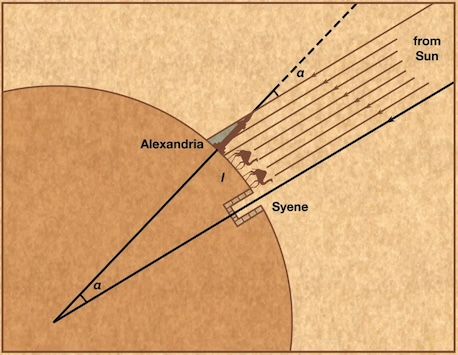
\includegraphics[scale=0.35]{img/eratosthenes-earth}}
 \subcaptionbox{太阳照射亚历山大的角度为$\alpha$\label{fig:atan8}}{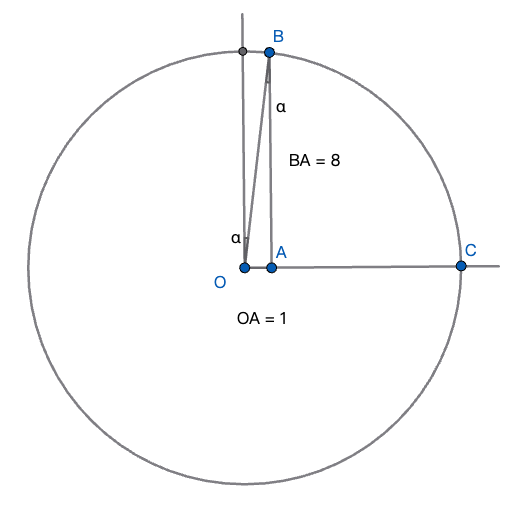
\includegraphics[scale=0.32]{img/atan8}}
 \caption{埃拉托斯特尼测量地球}
\end{figure}

夏至正午时刻,太阳直射北回归线,因此阳光可以射入赛印城的井底。埃拉托色特尼可以通过\cref{fig:atan8}找出阳光照射亚历山大港的角度。
%% 这相当于今天高中数学中的反正切$\arctan(\frac{1}{8})$。
但当时古巴比伦的角度单位还没有传入古希腊,按照埃拉托斯特尼的说法,这个角度是圆的50分之一,合$7.2\degree$。太阳光是平行光。如果大地是球形的,那么赛印城和亚历山大到球心的张角,是太阳入射角的同位角(\cref{fig:eratosthenes-earth}中标有$\alpha$的两个角),也是圆的50分之一。所以赛印城到亚历山大之间的距离就是地球周长的50分之一。这样算来,地球的周长就是$50 \times 5000 = 250000$斯塔提雅,约合$250 \times 158 = 39500 \approx 4$万千米。而今天人们通过人造卫星测得地球赤道长度为40075千米。埃拉托色特尼的著作没有流传到今天,我们从古希腊数学家帕普斯等人的记述中了解到他的具体测量方法。埃拉托色特尼约在公元前235年起任亚历山大图书馆馆长,他对地球的测量发生在这一时期\cite{Walkup2005}。赛印城到亚历山大的距离是一个关键,5000斯塔蒂亚无疑是一个大致数字。埃拉托斯特尼可能通过多种途径核证该距离,包括询问往来的商人以及测量地图。赛印城和亚历山大港都是尼罗河沿岸城市,尼罗河有规律的每年泛滥,埃及人因此每年在泛滥后重新丈量尼罗河沿线的土地并更新地图。此外,古希腊的斯塔蒂亚到底有多长学者们也有不同的观点。无论如何,埃拉托色特尼在2000年前的伟大推理和计算无疑是惊人的。

\begin{figure}[htbp]
 \centering
 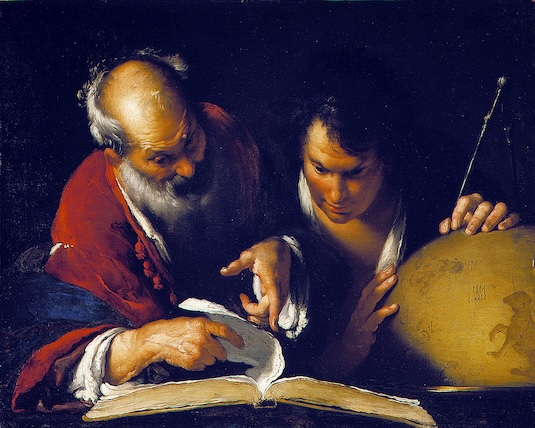
\includegraphics[scale=0.35]{img/eratosthenes}
 % https://commons.wikimedia.org/wiki/File:Eratosthenes_Teaching_in_Alexandria_(Bernardo_Strozzi,_Montreal).jpg
 \caption{贝尔纳多·斯特罗齐于1635年创作的油画:在亚历山大教学的埃拉托色特尼}
 \label{fig:eratosthenes}
\end{figure}

马其顿国王亚历山大大帝征服埃及后,兴建了以他命名的城市亚历山大港,成为了希腊化时代的文化和学术中心。埃拉托色特尼测量地球的壮举通常被认为是体现古希腊几何学力量的典范。古希腊并没有位值制计数系统(见第1章),但却发展出了严密的推理和几何学传统。正是在把数和几何学结合后,古希腊人\underdot{发现}了无理数,使得数的大家庭又得到了一次扩充。

\section{万物皆数}
音乐与数似乎毫无关联,但毕达哥拉斯却发现了它们背后竟有奇妙的规律。他从中得到启发并大胆推测“万物皆数”(All is number),认为世间万物都可以用数或数的比例来理解。毕达哥拉斯可以说是用数探索世间万物的第一人。他出生于希腊的萨摩斯(Samos)岛,年轻时他曾去米利都(Miletus)向古希腊哲学的奠基人泰勒斯(Thales)学习。在泰勒斯的建议下,毕达哥拉斯于公元535年前往埃及学习数学。公元前525年,波斯帝国征服了埃及,他被俘并随军向东到达了巴比伦。毕达哥拉斯得以向巴比伦人学习数学和天文知识。或许后来他还到达了更远的印度。不论到了哪里,毕达哥拉斯都不断向有学问的人请教,丰富自己的见解。重要的是,他不仅刻苦学习,而且更善于思考。在经过兼收并蓄、汲取各家之长后,毕达哥拉斯形成并完善了自己的思想\cite{HanXueTao16}。

经历了漫长的在外游历后,年近半百的毕达哥拉斯返回了故乡萨默斯并开始讲学。公元前520年左右,也许为了摆脱当地的暴政,毕达哥拉斯移居到了意大利南部的克罗顿(Croton)发展。在那里他赢得了人们的信任与景仰并形成了自己的学派。毕达哥拉斯的弟子中还有女性,学派把主要精力都用来研究天文、几何、数论、音乐这四门学科。它们被称为四术(quadrivium),影响了欧洲教育两千多年\cite{StepanovRose15}。四术体现了毕达哥拉斯万物皆数的哲学思想:星体的运动与几何对应,而几何又以数为基础,数字还可以衍生出音乐(见第3章)。关于毕达哥拉斯去世有多种说法。他领导的学派具有很高的声誉和政治影响,引起了敌对派的忌恨。约公元前497年,学派在克罗顿的活动场所遭到破坏。有人认为毕达哥拉斯被暴徒杀害,也有人说他逃到梅塔蓬图姆(Metapontum)并度过余生\cite{MKlein1972}。

\index{形数(figurate number)}
毕达哥拉斯学派研究数字,认为数与数、数与自然之间存在着神秘关系。这开启了数学的重要分支——数论。学派对正整数进行了分类,定义了奇数、偶数、素数、合数等。他们通过在地上摆小石子来研究数字,英文的计算calculus一词就是从希腊文“石子”衍生出的\cite{HanXueTao16}。当把石子按照某种几何图形摆放时,就得到了形数(figurate number)。

\begin{figure}[htbp]
%\begin{wrapfigure}{R}{0.4\textwidth}
\centering
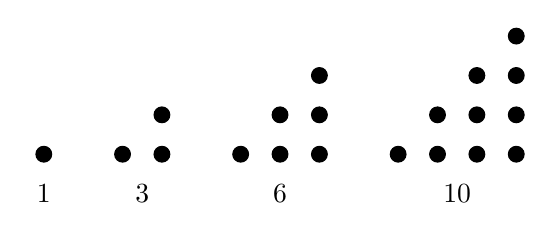
\begin{tikzpicture}[scale=0.5]
\filldraw (0, 0) circle (0.2);
\draw (0, -1) node{1};
\filldraw (2, 0) circle (0.2)
          (3, 0) circle (0.2)   (3, 1) circle (0.2);
\draw (2.5, -1) node{3};
\filldraw (5, 0) circle (0.2)
          (6, 0) circle (0.2)   (6, 1) circle (0.2)
          (7, 0) circle (0.2)   (7, 1) circle (0.2)   (7, 2) circle (0.2);
\draw (6, -1) node{6};
\filldraw (9, 0) circle (0.2)
          (10, 0) circle (0.2)    (10, 1) circle (0.2)
          (11, 0) circle (0.2)    (11, 1) circle (0.2)    (11, 2) circle (0.2)
          (12, 0) circle (0.2)    (12, 1) circle (0.2)    (12, 2) circle (0.2)    (12, 3) circle (0.2);
\draw (10.5, -1) node{10};
\end{tikzpicture}
\caption{三角形数(triangular number)}
\label{fig:triangular-num}
%\end{wrapfigure}
\end{figure}

\begin{figure}[htbp]
%\begin{wrapfigure}{R}{0.4\textwidth}
\centering
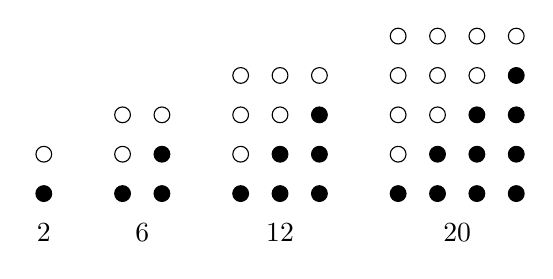
\begin{tikzpicture}[scale=0.5]
\draw (0, 1) circle (0.2);
\filldraw (0, 0) circle (0.2);
\draw (0, -1) node{2};

\draw (2, 1) circle (0.2)   (2, 2) circle (0.2)
      (3, 2) circle (0.2);
\filldraw (2, 0) circle (0.2)
          (3, 0) circle (0.2)   (3, 1) circle (0.2);
\draw (2.5, -1) node{6};

\draw (5, 1) circle (0.2)   (5, 2) circle (0.2)   (5, 3) circle (0.2)
      (6, 2) circle (0.2)   (6, 3) circle (0.2)
      (7, 3) circle (0.2);
\filldraw (5, 0) circle (0.2)
          (6, 0) circle (0.2)   (6, 1) circle (0.2)
          (7, 0) circle (0.2)   (7, 1) circle (0.2)   (7, 2) circle (0.2);
\draw (6, -1) node{12};

\draw (9, 1) circle (0.2)   (9, 2) circle (0.2)   (9, 3) circle (0.2)   (9, 4) circle (0.2)
      (10, 2) circle (0.2)   (10, 3) circle (0.2)   (10, 4) circle (0.2)
      (11, 3) circle (0.2)   (11, 4) circle (0.2)
      (12, 4) circle (0.2);
\filldraw (9, 0) circle (0.2)
          (10, 0) circle (0.2)    (10, 1) circle (0.2)
          (11, 0) circle (0.2)    (11, 1) circle (0.2)    (11, 2) circle (0.2)
          (12, 0) circle (0.2)    (12, 1) circle (0.2)    (12, 2) circle (0.2)    (12, 3) circle (0.2);
\draw (10.5, -1) node{20};
\end{tikzpicture}
\caption{长方形数(oblong number)}
\label{fig:oblong-num}
%\end{wrapfigure}
\end{figure}

\cref{fig:triangular-num}和\cref{fig:oblong-num}分别是三角形数和长方形数。容易看出,每个长方形数都对应三角形数的二倍,而三角形数又是前$n$个正整数之和,这样就得到了正整数累加的求和公式:

\[
1 + 2 + 3 + ... + n = \frac{1}{2}n(n+1)
\]

毕达哥拉斯学派还观察到,所有的奇数可以表示成折尺形(或称为“磬折形”)\footnote{gnomon这个字在巴比伦人的原意可能是指日晷上的直杆,用它的阴影来指示时刻。在毕达哥拉斯时代,gnomon指木匠用的方尺。它还表示从正方形的一角切掉一个小正方形后剩余的图形。以后欧几里得又把正方形扩展到平行四边形\citepage[26页]{MKlein1972}。},如\cref{fig:gnomon-num},而前$n$个折尺形可以拼成一个正方形,如\cref{fig:square-num}。这样他们就发现了前$n$个正奇数的求和公式:

\[
1 + 3 + 5 + ... + (2n - 1) = n^2
\]

\begin{figure}[htbp]
%\begin{wrapfigure}{R}{0.4\textwidth}
\centering
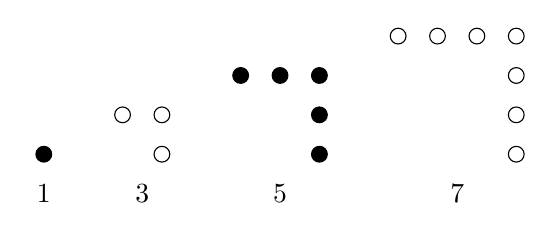
\begin{tikzpicture}[scale=0.5]
\filldraw (0, 0) circle (0.2);
\draw (0, -1) node{1};

\draw (2, 1) circle (0.2)
      (3, 0) circle (0.2)   (3, 1) circle (0.2);
\draw (2.5, -1) node{3};

\filldraw (5, 2) circle (0.2)   (6, 2) circle (0.2)   (7, 2) circle (0.2)
          (7, 0) circle (0.2)   (7, 1) circle (0.2);
\draw (6, -1) node{5};

\draw (9, 3) circle (0.2)   (10, 3) circle (0.2)   (11, 3) circle (0.2)   (12, 3) circle (0.2)
      (12, 0) circle (0.2)    (12, 1) circle (0.2)    (12, 2) circle (0.2);
\draw (10.5, -1) node{7};
\end{tikzpicture}
\caption{折尺形数(gnomon number)}
\label{fig:gnomon-num}
%\end{wrapfigure}
\end{figure}

\begin{figure}[htbp]
%\begin{wrapfigure}{R}{0.4\textwidth}
\centering
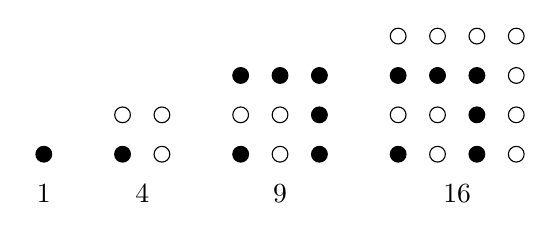
\begin{tikzpicture}[scale=0.5]
\filldraw (0, 0) circle (0.2);
\draw (0, -1) node{1};

\filldraw (2, 0) circle (0.2);
\draw (2, 1) circle (0.2)
      (3, 0) circle (0.2)   (3, 1) circle (0.2);
\draw (2.5, -1) node{4};

\filldraw (5, 0) circle (0.2);
\draw (5, 1) circle (0.2)
      (6, 0) circle (0.2)   (6, 1) circle (0.2);
\filldraw (5, 2) circle (0.2)   (6, 2) circle (0.2)   (7, 2) circle (0.2)
          (7, 0) circle (0.2)   (7, 1) circle (0.2);
\draw (6, -1) node{9};

\filldraw (9, 0) circle (0.2);
\draw (9, 1) circle (0.2)
      (10, 0) circle (0.2)   (10, 1) circle (0.2);
\filldraw (9, 2) circle (0.2)   (10, 2) circle (0.2)   (11, 2) circle (0.2)
          (11, 0) circle (0.2)   (11, 1) circle (0.2);
\draw (9, 3) circle (0.2)   (10, 3) circle (0.2)   (11, 3) circle (0.2)   (12, 3) circle (0.2)
      (12, 0) circle (0.2)    (12, 1) circle (0.2)    (12, 2) circle (0.2);
\draw (10.5, -1) node{16};
\end{tikzpicture}
\caption{正方形数(square number)与折尺形数的关系}
\label{fig:square-num}
%\end{wrapfigure}
\end{figure}

就这样,毕达哥拉斯学派把几何形状也建立在了数的基础上。他们热衷与用数去解释更多的现象,并相信宇宙的本质就在于“数的和谐”,由此出发,毕达哥拉斯学派试图发展一套以数字为基础的理论,使得几何学可以建立在该理论之上。

\section{勾股定理}
毕达哥拉斯学派最著名的发现当属勾股定理,在西方叫做“毕达哥拉斯定理”。据说毕达哥拉斯对他发现的这个定理及其证明极为高兴,为此献祭了一百头公牛庆贺。但脍炙人口的传说故事往往不真实。毕达哥拉斯学派对团体成员有着极为严格的戒律,任何人的研究发现都归学派所有并必须保密。我们所知的以“毕达哥拉斯”命名的成果大都来自学派内的佚名作者。勾股定理并非孤立成果,各个文明都各自独立发现了它。如第3章中的\cref{fig:babylonian-yale}所示,这块古巴比伦泥板的时间大约是公元前1900年~1600年,此外人们还发现了刻有勾股数表的泥板。古埃及的测量员绳子作为软尺(称为拉绳人)。相传他们在绳上打结,把全长分成长度为3比4比5的三段,然后用来形成直角三角形。但这个说法没有文献证实\citepage[16页]{MKlein1972}。古印度数学家包德哈亚那(Baudhayana,生活在公元前800年到公元前400年间)的著作《绳法经》(Śulba Sutra)也提到了这个定理。在古代中国,成书于公元前一世纪的《周髀算经》中载有西周时代(约公元前11世纪)周公和商高的一段对话,其中提到“勾三、股四、弦五”\footnote{商高说:“……故折矩,勾广三,股修四,经隅五。”},故在中国称之为“勾股定理”。《九章算术》的注解中载有三国时代的赵爽和魏晋时刘徽给出的勾股定理证明\footnote{对赵爽和刘徽给出的究竟是严格意义的证明还是某种程度的解释历来有不同观点。}。

这一定理自提出以来,吸引了无数聪明的头脑对它进行证明,包括意大利文艺复兴时期的全才达芬奇和美国总统加菲尔德。在4000年的时间里,诞生了超过300多种不同的证明。如今在中学数学课堂上就至少有“赵爽弦图”(见\cref{fig:cms-zhaoshuang}),传说中的“毕达哥拉斯证法”和《原本》证法。

\begin{figure}[htbp]
 \centering
 \subcaptionbox{中国数学会会徽\label{fig:cms-logo}}{
\includegraphics[scale=0.5]{img/cms}} \quad
 \subcaptionbox{赵爽弦图\label{fig:zhaoshuang}}{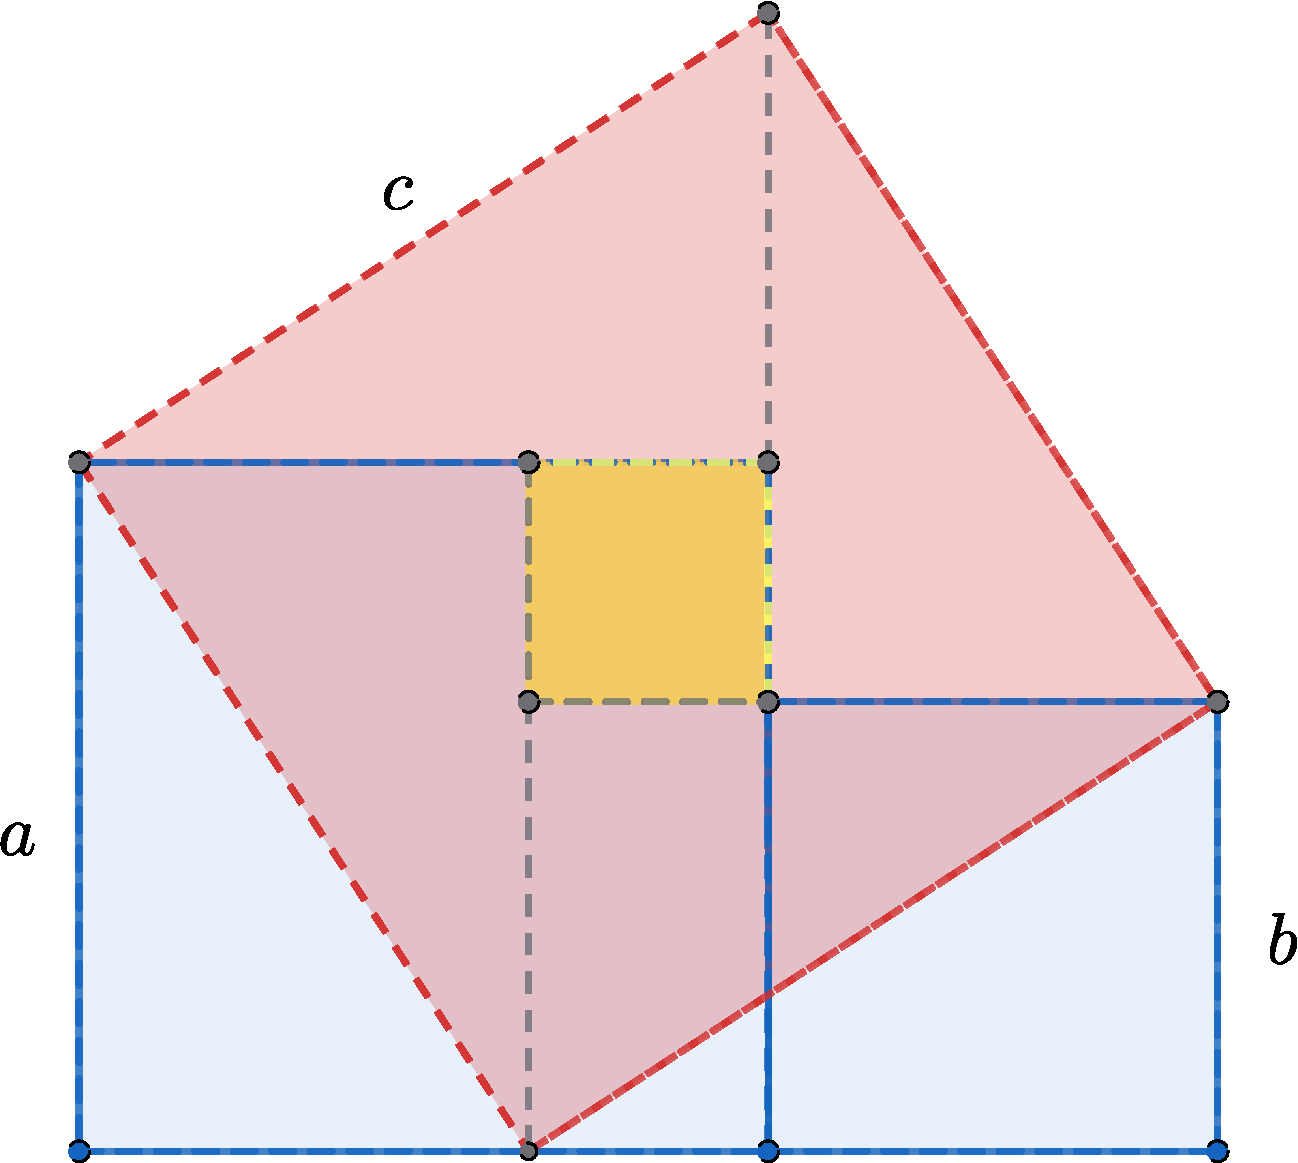
\includegraphics[scale=0.2]{img/zhaoshuang}}
 \caption{赵爽弦图成为了2002年在北京召开的国际数学家大会和中国数学会的会徽。\label{fig:cms-zhaoshuang}}
\end{figure}


\section{数论}
Euclid's proof to the Pythagoras triples.
Euclid and Elements
Perfect numbers and Even perfect numbers theorem (Euclid), Fermat numbers and Mersenne primes.
毕达哥拉斯学派并非纯粹的学术团体。学派信奉数字神秘主义,
他们发现某些数的所有真因子\footnote{真因子是小于数本身的因子}之和恰好等于这个数本身,于是将其命名为完全数,并成功地找到两个\footnote{一说为完美数。经过欧几里得与欧拉的进一步工作,揭示了偶完全数的特征以及完全数和梅森素数的关系。到2018年,人们借助计算机发现了前50个梅森素数和完全数。}。最小的完全数是6,因为6 = 1 + 2 + 3,下一个是28(等于1 + 2 + 4 + 7 + 14)。

\section{无理数}
Discovery of irrational number, square root of 2 and n.
Compass and ruler construction I
Golden ration and Fibonacci series.

\section{欧几里得算法}
Euclidean algorithm,
It's extension and Bezout identity.
Geometric meaning of Euclidean algorithm.
Continue fraction and Euclidean algorithm.
Uncommensurable and irrational numbers, (Elements)

\section{更多的无理数}
Compass and ruler construction II,

polygon construction (pentagon, 17-gon)

Solving polygon construction with number theory, Fermat numbers, Perfect numbers, and Wantzel theorem.

\section{圆周率}
pi as an irrational number

\section{思想之剑}
Dedekind cut

\ifx\wholebook\relax \else
\section{参考答案}
\shipoutAnswer

\begin{thebibliography}{99}
\subimport{inc/}{bib-zh-cn}
\end{thebibliography}

\expandafter\enddocument
\fi
